% Created by tikzDevice version 0.11 on 2018-08-06 22:54:01
% !TEX encoding = UTF-8 Unicode
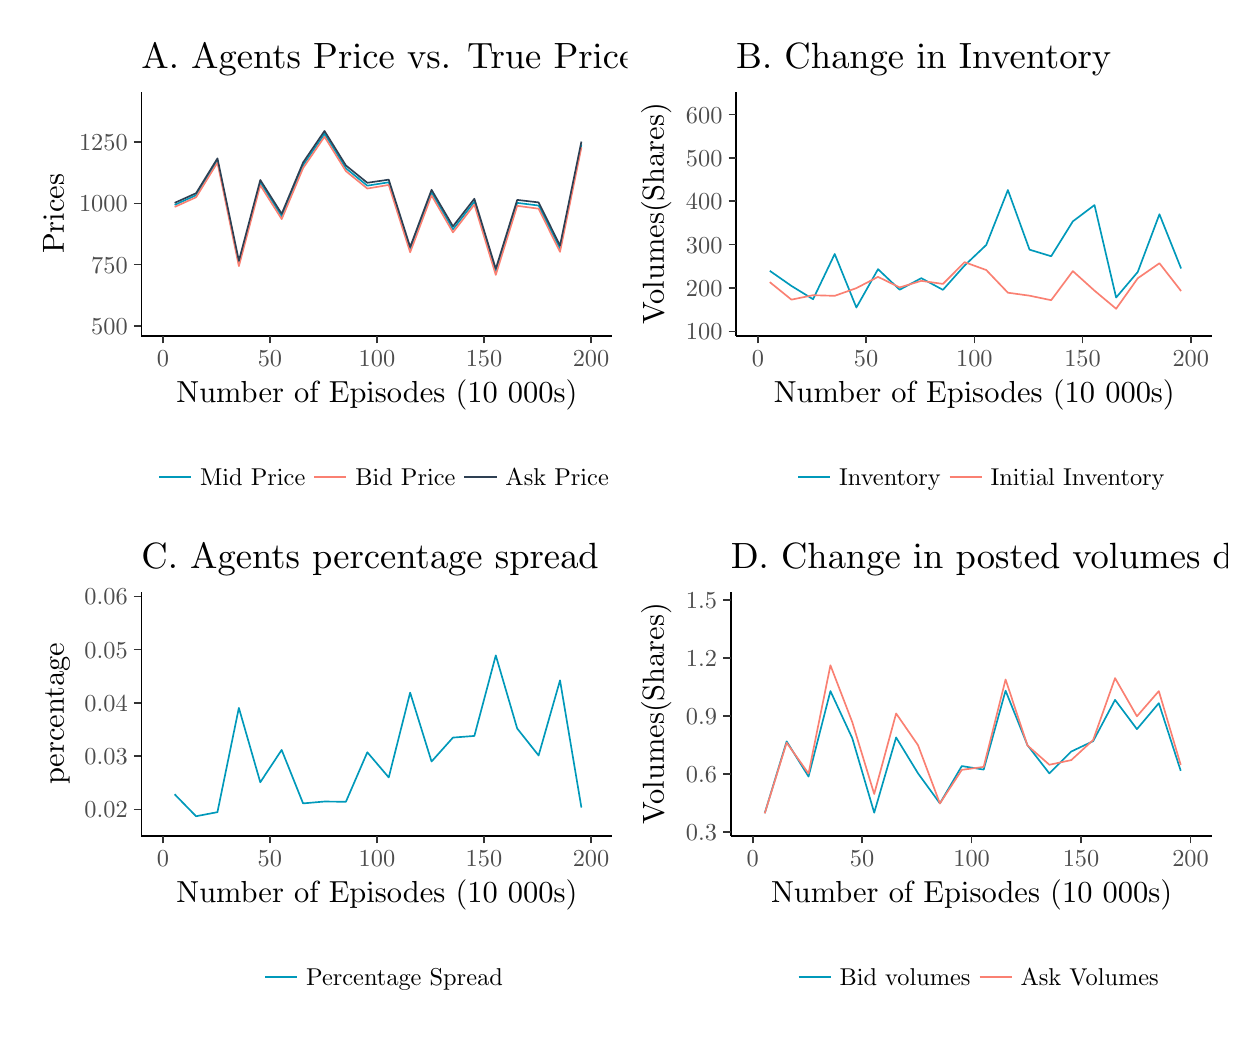
\begin{tikzpicture}[x=1pt,y=1pt]
\definecolor{fillColor}{RGB}{255,255,255}
\path[use as bounding box,fill=fillColor,fill opacity=0.00] (0,0) rectangle (433.62,361.35);
\begin{scope}
\path[clip] (  0.00,180.67) rectangle (216.81,361.35);
\definecolor{drawColor}{RGB}{255,255,255}
\definecolor{fillColor}{RGB}{255,255,255}

\path[draw=drawColor,line width= 0.6pt,line join=round,line cap=round,fill=fillColor] (  0.00,180.67) rectangle (216.81,361.35);
\end{scope}
\begin{scope}
\path[clip] ( 41.12,249.98) rectangle (211.31,338.21);
\definecolor{fillColor}{RGB}{255,255,255}

\path[fill=fillColor] ( 41.12,249.98) rectangle (211.31,338.21);
\definecolor{drawColor}{RGB}{0,153,186}

\path[draw=drawColor,line width= 0.6pt,line join=round] ( 53.11,297.30) --
	( 60.85,300.80) --
	( 68.58,313.37) --
	( 76.32,276.14) --
	( 84.06,305.36) --
	( 91.79,293.14) --
	( 99.53,311.64) --
	(107.26,322.98) --
	(115.00,310.53) --
	(122.73,304.25) --
	(130.47,305.48) --
	(138.21,281.14) --
	(145.94,301.76) --
	(153.68,288.47) --
	(161.41,298.47) --
	(169.15,273.11) --
	(176.89,298.04) --
	(184.62,297.07) --
	(192.36,281.49) --
	(200.09,319.16);
\definecolor{drawColor}{RGB}{250,128,114}

\path[draw=drawColor,line width= 0.6pt,line join=round] ( 53.11,296.56) --
	( 60.85,300.06) --
	( 68.58,312.62) --
	( 76.32,275.17) --
	( 84.06,304.41) --
	( 91.79,292.18) --
	( 99.53,310.63) --
	(107.26,321.95) --
	(115.00,309.50) --
	(122.73,303.21) --
	(130.47,304.52) --
	(138.21,280.19) --
	(145.94,300.75) --
	(153.68,287.38) --
	(161.41,297.42) --
	(169.15,272.01) --
	(176.89,296.97) --
	(184.62,295.93) --
	(192.36,280.35) --
	(200.09,318.12);
\definecolor{drawColor}{RGB}{46,64,83}

\path[draw=drawColor,line width= 0.6pt,line join=round] ( 53.11,298.04) --
	( 60.85,301.53) --
	( 68.58,314.12) --
	( 76.32,277.10) --
	( 84.06,306.30) --
	( 91.79,294.09) --
	( 99.53,312.65) --
	(107.26,324.02) --
	(115.00,311.55) --
	(122.73,305.30) --
	(130.47,306.43) --
	(138.21,282.10) --
	(145.94,302.76) --
	(153.68,289.57) --
	(161.41,299.52) --
	(169.15,274.22) --
	(176.89,299.11) --
	(184.62,298.21) --
	(192.36,282.63) --
	(200.09,320.20);
\end{scope}
\begin{scope}
\path[clip] (  0.00,  0.00) rectangle (433.62,361.35);
\definecolor{drawColor}{RGB}{0,0,0}

\path[draw=drawColor,line width= 0.6pt,line join=round] ( 41.12,249.98) --
	( 41.12,338.21);
\end{scope}
\begin{scope}
\path[clip] (  0.00,  0.00) rectangle (433.62,361.35);
\definecolor{drawColor}{gray}{0.30}

\node[text=drawColor,anchor=base east,inner sep=0pt, outer sep=0pt, scale=  0.88] at ( 36.17,250.57) {500};

\node[text=drawColor,anchor=base east,inner sep=0pt, outer sep=0pt, scale=  0.88] at ( 36.17,272.68) {750};

\node[text=drawColor,anchor=base east,inner sep=0pt, outer sep=0pt, scale=  0.88] at ( 36.17,294.79) {1000};

\node[text=drawColor,anchor=base east,inner sep=0pt, outer sep=0pt, scale=  0.88] at ( 36.17,316.90) {1250};
\end{scope}
\begin{scope}
\path[clip] (  0.00,  0.00) rectangle (433.62,361.35);
\definecolor{drawColor}{gray}{0.20}

\path[draw=drawColor,line width= 0.6pt,line join=round] ( 38.37,253.60) --
	( 41.12,253.60);

\path[draw=drawColor,line width= 0.6pt,line join=round] ( 38.37,275.71) --
	( 41.12,275.71);

\path[draw=drawColor,line width= 0.6pt,line join=round] ( 38.37,297.82) --
	( 41.12,297.82);

\path[draw=drawColor,line width= 0.6pt,line join=round] ( 38.37,319.93) --
	( 41.12,319.93);
\end{scope}
\begin{scope}
\path[clip] (  0.00,  0.00) rectangle (433.62,361.35);
\definecolor{drawColor}{RGB}{0,0,0}

\path[draw=drawColor,line width= 0.6pt,line join=round] ( 41.12,249.98) --
	(211.31,249.98);
\end{scope}
\begin{scope}
\path[clip] (  0.00,  0.00) rectangle (433.62,361.35);
\definecolor{drawColor}{gray}{0.20}

\path[draw=drawColor,line width= 0.6pt,line join=round] ( 48.86,247.23) --
	( 48.86,249.98);

\path[draw=drawColor,line width= 0.6pt,line join=round] ( 87.54,247.23) --
	( 87.54,249.98);

\path[draw=drawColor,line width= 0.6pt,line join=round] (126.22,247.23) --
	(126.22,249.98);

\path[draw=drawColor,line width= 0.6pt,line join=round] (164.90,247.23) --
	(164.90,249.98);

\path[draw=drawColor,line width= 0.6pt,line join=round] (203.57,247.23) --
	(203.57,249.98);
\end{scope}
\begin{scope}
\path[clip] (  0.00,  0.00) rectangle (433.62,361.35);
\definecolor{drawColor}{gray}{0.30}

\node[text=drawColor,anchor=base,inner sep=0pt, outer sep=0pt, scale=  0.88] at ( 48.86,238.97) {0};

\node[text=drawColor,anchor=base,inner sep=0pt, outer sep=0pt, scale=  0.88] at ( 87.54,238.97) {50};

\node[text=drawColor,anchor=base,inner sep=0pt, outer sep=0pt, scale=  0.88] at (126.22,238.97) {100};

\node[text=drawColor,anchor=base,inner sep=0pt, outer sep=0pt, scale=  0.88] at (164.90,238.97) {150};

\node[text=drawColor,anchor=base,inner sep=0pt, outer sep=0pt, scale=  0.88] at (203.57,238.97) {200};
\end{scope}
\begin{scope}
\path[clip] (  0.00,  0.00) rectangle (433.62,361.35);
\definecolor{drawColor}{RGB}{0,0,0}

\node[text=drawColor,anchor=base,inner sep=0pt, outer sep=0pt, scale=  1.10] at (126.22,225.89) {Number of Episodes (10 000s)};
\end{scope}
\begin{scope}
\path[clip] (  0.00,  0.00) rectangle (433.62,361.35);
\definecolor{drawColor}{RGB}{0,0,0}

\node[text=drawColor,rotate= 90.00,anchor=base,inner sep=0pt, outer sep=0pt, scale=  1.10] at ( 13.08,294.10) {Prices};
\end{scope}
\begin{scope}
\path[clip] (  0.00,  0.00) rectangle (433.62,361.35);
\definecolor{fillColor}{RGB}{255,255,255}

\path[fill=fillColor] ( 36.74,186.17) rectangle (215.69,212.01);
\end{scope}
\begin{scope}
\path[clip] (  0.00,  0.00) rectangle (433.62,361.35);
\definecolor{drawColor}{RGB}{0,153,186}

\path[draw=drawColor,line width= 0.6pt,line join=round] ( 47.49,199.09) -- ( 59.05,199.09);
\end{scope}
\begin{scope}
\path[clip] (  0.00,  0.00) rectangle (433.62,361.35);
\definecolor{drawColor}{RGB}{250,128,114}

\path[draw=drawColor,line width= 0.6pt,line join=round] (103.58,199.09) -- (115.15,199.09);
\end{scope}
\begin{scope}
\path[clip] (  0.00,  0.00) rectangle (433.62,361.35);
\definecolor{drawColor}{RGB}{46,64,83}

\path[draw=drawColor,line width= 0.6pt,line join=round] (157.84,199.09) -- (169.41,199.09);
\end{scope}
\begin{scope}
\path[clip] (  0.00,  0.00) rectangle (433.62,361.35);
\definecolor{drawColor}{RGB}{0,0,0}

\node[text=drawColor,anchor=base west,inner sep=0pt, outer sep=0pt, scale=  0.88] at ( 62.30,196.06) {Mid Price};
\end{scope}
\begin{scope}
\path[clip] (  0.00,  0.00) rectangle (433.62,361.35);
\definecolor{drawColor}{RGB}{0,0,0}

\node[text=drawColor,anchor=base west,inner sep=0pt, outer sep=0pt, scale=  0.88] at (118.40,196.06) {Bid Price};
\end{scope}
\begin{scope}
\path[clip] (  0.00,  0.00) rectangle (433.62,361.35);
\definecolor{drawColor}{RGB}{0,0,0}

\node[text=drawColor,anchor=base west,inner sep=0pt, outer sep=0pt, scale=  0.88] at (172.66,196.06) {Ask Price};
\end{scope}
\begin{scope}
\path[clip] (  0.00,  0.00) rectangle (433.62,361.35);
\definecolor{drawColor}{RGB}{0,0,0}

\node[text=drawColor,anchor=base west,inner sep=0pt, outer sep=0pt, scale=  1.32] at ( 41.12,346.76) {A. Agents Price vs. True Price};
\end{scope}
\begin{scope}
\path[clip] (  0.00,  0.00) rectangle (216.81,180.67);
\definecolor{drawColor}{RGB}{255,255,255}
\definecolor{fillColor}{RGB}{255,255,255}

\path[draw=drawColor,line width= 0.6pt,line join=round,line cap=round,fill=fillColor] (  0.00, -0.00) rectangle (216.81,180.67);
\end{scope}
\begin{scope}
\path[clip] ( 41.11, 69.30) rectangle (211.31,157.54);
\definecolor{fillColor}{RGB}{255,255,255}

\path[fill=fillColor] ( 41.11, 69.30) rectangle (211.31,157.54);
\definecolor{drawColor}{RGB}{0,153,186}

\path[draw=drawColor,line width= 0.6pt,line join=round] ( 53.10, 84.34) --
	( 60.84, 76.40) --
	( 68.57, 77.88) --
	( 76.31,115.56) --
	( 84.05, 88.68) --
	( 91.78,100.36) --
	( 99.52, 81.04) --
	(107.26, 81.72) --
	(114.99, 81.62) --
	(122.73, 99.52) --
	(130.47, 90.42) --
	(138.20,121.08) --
	(145.94, 96.17) --
	(153.67,104.82) --
	(161.41,105.42) --
	(169.15,134.52) --
	(176.88,108.12) --
	(184.62, 98.36) --
	(192.36,125.51) --
	(200.09, 79.53);
\end{scope}
\begin{scope}
\path[clip] (  0.00,  0.00) rectangle (433.62,361.35);
\definecolor{drawColor}{RGB}{0,0,0}

\path[draw=drawColor,line width= 0.6pt,line join=round] ( 41.11, 69.30) --
	( 41.11,157.54);
\end{scope}
\begin{scope}
\path[clip] (  0.00,  0.00) rectangle (433.62,361.35);
\definecolor{drawColor}{gray}{0.30}

\node[text=drawColor,anchor=base east,inner sep=0pt, outer sep=0pt, scale=  0.88] at ( 36.16, 75.85) {0.02};

\node[text=drawColor,anchor=base east,inner sep=0pt, outer sep=0pt, scale=  0.88] at ( 36.16, 95.09) {0.03};

\node[text=drawColor,anchor=base east,inner sep=0pt, outer sep=0pt, scale=  0.88] at ( 36.16,114.32) {0.04};

\node[text=drawColor,anchor=base east,inner sep=0pt, outer sep=0pt, scale=  0.88] at ( 36.16,133.56) {0.05};

\node[text=drawColor,anchor=base east,inner sep=0pt, outer sep=0pt, scale=  0.88] at ( 36.16,152.80) {0.06};
\end{scope}
\begin{scope}
\path[clip] (  0.00,  0.00) rectangle (433.62,361.35);
\definecolor{drawColor}{gray}{0.20}

\path[draw=drawColor,line width= 0.6pt,line join=round] ( 38.36, 78.89) --
	( 41.11, 78.89);

\path[draw=drawColor,line width= 0.6pt,line join=round] ( 38.36, 98.12) --
	( 41.11, 98.12);

\path[draw=drawColor,line width= 0.6pt,line join=round] ( 38.36,117.36) --
	( 41.11,117.36);

\path[draw=drawColor,line width= 0.6pt,line join=round] ( 38.36,136.59) --
	( 41.11,136.59);

\path[draw=drawColor,line width= 0.6pt,line join=round] ( 38.36,155.83) --
	( 41.11,155.83);
\end{scope}
\begin{scope}
\path[clip] (  0.00,  0.00) rectangle (433.62,361.35);
\definecolor{drawColor}{RGB}{0,0,0}

\path[draw=drawColor,line width= 0.6pt,line join=round] ( 41.11, 69.30) --
	(211.31, 69.30);
\end{scope}
\begin{scope}
\path[clip] (  0.00,  0.00) rectangle (433.62,361.35);
\definecolor{drawColor}{gray}{0.20}

\path[draw=drawColor,line width= 0.6pt,line join=round] ( 48.85, 66.55) --
	( 48.85, 69.30);

\path[draw=drawColor,line width= 0.6pt,line join=round] ( 87.53, 66.55) --
	( 87.53, 69.30);

\path[draw=drawColor,line width= 0.6pt,line join=round] (126.21, 66.55) --
	(126.21, 69.30);

\path[draw=drawColor,line width= 0.6pt,line join=round] (164.89, 66.55) --
	(164.89, 69.30);

\path[draw=drawColor,line width= 0.6pt,line join=round] (203.57, 66.55) --
	(203.57, 69.30);
\end{scope}
\begin{scope}
\path[clip] (  0.00,  0.00) rectangle (433.62,361.35);
\definecolor{drawColor}{gray}{0.30}

\node[text=drawColor,anchor=base,inner sep=0pt, outer sep=0pt, scale=  0.88] at ( 48.85, 58.29) {0};

\node[text=drawColor,anchor=base,inner sep=0pt, outer sep=0pt, scale=  0.88] at ( 87.53, 58.29) {50};

\node[text=drawColor,anchor=base,inner sep=0pt, outer sep=0pt, scale=  0.88] at (126.21, 58.29) {100};

\node[text=drawColor,anchor=base,inner sep=0pt, outer sep=0pt, scale=  0.88] at (164.89, 58.29) {150};

\node[text=drawColor,anchor=base,inner sep=0pt, outer sep=0pt, scale=  0.88] at (203.57, 58.29) {200};
\end{scope}
\begin{scope}
\path[clip] (  0.00,  0.00) rectangle (433.62,361.35);
\definecolor{drawColor}{RGB}{0,0,0}

\node[text=drawColor,anchor=base,inner sep=0pt, outer sep=0pt, scale=  1.10] at (126.21, 45.22) {Number of Episodes (10 000s)};
\end{scope}
\begin{scope}
\path[clip] (  0.00,  0.00) rectangle (433.62,361.35);
\definecolor{drawColor}{RGB}{0,0,0}

\node[text=drawColor,rotate= 90.00,anchor=base,inner sep=0pt, outer sep=0pt, scale=  1.10] at ( 13.08,113.42) {percentage};
\end{scope}
\begin{scope}
\path[clip] (  0.00,  0.00) rectangle (433.62,361.35);
\definecolor{fillColor}{RGB}{255,255,255}

\path[fill=fillColor] ( 75.06,  5.50) rectangle (177.36, 31.34);
\end{scope}
\begin{scope}
\path[clip] (  0.00,  0.00) rectangle (433.62,361.35);
\definecolor{drawColor}{RGB}{0,153,186}

\path[draw=drawColor,line width= 0.6pt,line join=round] ( 85.81, 18.42) -- ( 97.37, 18.42);
\end{scope}
\begin{scope}
\path[clip] (  0.00,  0.00) rectangle (433.62,361.35);
\definecolor{drawColor}{RGB}{0,0,0}

\node[text=drawColor,anchor=base west,inner sep=0pt, outer sep=0pt, scale=  0.88] at (100.63, 15.39) {Percentage Spread};
\end{scope}
\begin{scope}
\path[clip] (  0.00,  0.00) rectangle (433.62,361.35);
\definecolor{drawColor}{RGB}{0,0,0}

\node[text=drawColor,anchor=base west,inner sep=0pt, outer sep=0pt, scale=  1.32] at ( 41.11,166.08) {C. Agents percentage spread};
\end{scope}
\begin{scope}
\path[clip] (216.81,180.67) rectangle (433.62,361.35);
\definecolor{drawColor}{RGB}{255,255,255}
\definecolor{fillColor}{RGB}{255,255,255}

\path[draw=drawColor,line width= 0.6pt,line join=round,line cap=round,fill=fillColor] (216.81,180.67) rectangle (433.62,361.35);
\end{scope}
\begin{scope}
\path[clip] (256.03,249.98) rectangle (428.12,338.21);
\definecolor{fillColor}{RGB}{255,255,255}

\path[fill=fillColor] (256.03,249.98) rectangle (428.12,338.21);
\definecolor{drawColor}{RGB}{0,153,186}

\path[draw=drawColor,line width= 0.6pt,line join=round] (268.16,273.48) --
	(275.98,268.03) --
	(283.80,263.22) --
	(291.62,279.56) --
	(299.45,260.22) --
	(307.27,274.07) --
	(315.09,266.66) --
	(322.91,270.83) --
	(330.73,266.61) --
	(338.56,275.41) --
	(346.38,282.83) --
	(354.20,302.67) --
	(362.02,281.13) --
	(369.84,278.75) --
	(377.67,291.35) --
	(385.49,297.25) --
	(393.31,263.83) --
	(401.13,273.08) --
	(408.96,293.93) --
	(416.78,274.33);
\definecolor{drawColor}{RGB}{250,128,114}

\path[draw=drawColor,line width= 0.6pt,line join=round] (268.16,269.40) --
	(275.98,263.07) --
	(283.80,264.67) --
	(291.62,264.45) --
	(299.45,267.23) --
	(307.27,271.30) --
	(315.09,267.48) --
	(322.91,269.86) --
	(330.73,268.75) --
	(338.56,276.61) --
	(346.38,273.77) --
	(354.20,265.58) --
	(362.02,264.50) --
	(369.84,262.87) --
	(377.67,273.38) --
	(385.49,266.32) --
	(393.31,259.78) --
	(401.13,270.80) --
	(408.96,276.22) --
	(416.78,266.19);
\end{scope}
\begin{scope}
\path[clip] (  0.00,  0.00) rectangle (433.62,361.35);
\definecolor{drawColor}{RGB}{0,0,0}

\path[draw=drawColor,line width= 0.6pt,line join=round] (256.03,249.98) --
	(256.03,338.21);
\end{scope}
\begin{scope}
\path[clip] (  0.00,  0.00) rectangle (433.62,361.35);
\definecolor{drawColor}{gray}{0.30}

\node[text=drawColor,anchor=base east,inner sep=0pt, outer sep=0pt, scale=  0.88] at (251.08,248.58) {100};

\node[text=drawColor,anchor=base east,inner sep=0pt, outer sep=0pt, scale=  0.88] at (251.08,264.24) {200};

\node[text=drawColor,anchor=base east,inner sep=0pt, outer sep=0pt, scale=  0.88] at (251.08,279.91) {300};

\node[text=drawColor,anchor=base east,inner sep=0pt, outer sep=0pt, scale=  0.88] at (251.08,295.57) {400};

\node[text=drawColor,anchor=base east,inner sep=0pt, outer sep=0pt, scale=  0.88] at (251.08,311.24) {500};

\node[text=drawColor,anchor=base east,inner sep=0pt, outer sep=0pt, scale=  0.88] at (251.08,326.90) {600};
\end{scope}
\begin{scope}
\path[clip] (  0.00,  0.00) rectangle (433.62,361.35);
\definecolor{drawColor}{gray}{0.20}

\path[draw=drawColor,line width= 0.6pt,line join=round] (253.28,251.61) --
	(256.03,251.61);

\path[draw=drawColor,line width= 0.6pt,line join=round] (253.28,267.27) --
	(256.03,267.27);

\path[draw=drawColor,line width= 0.6pt,line join=round] (253.28,282.94) --
	(256.03,282.94);

\path[draw=drawColor,line width= 0.6pt,line join=round] (253.28,298.60) --
	(256.03,298.60);

\path[draw=drawColor,line width= 0.6pt,line join=round] (253.28,314.27) --
	(256.03,314.27);

\path[draw=drawColor,line width= 0.6pt,line join=round] (253.28,329.94) --
	(256.03,329.94);
\end{scope}
\begin{scope}
\path[clip] (  0.00,  0.00) rectangle (433.62,361.35);
\definecolor{drawColor}{RGB}{0,0,0}

\path[draw=drawColor,line width= 0.6pt,line join=round] (256.03,249.98) --
	(428.12,249.98);
\end{scope}
\begin{scope}
\path[clip] (  0.00,  0.00) rectangle (433.62,361.35);
\definecolor{drawColor}{gray}{0.20}

\path[draw=drawColor,line width= 0.6pt,line join=round] (263.85,247.23) --
	(263.85,249.98);

\path[draw=drawColor,line width= 0.6pt,line join=round] (302.97,247.23) --
	(302.97,249.98);

\path[draw=drawColor,line width= 0.6pt,line join=round] (342.08,247.23) --
	(342.08,249.98);

\path[draw=drawColor,line width= 0.6pt,line join=round] (381.19,247.23) --
	(381.19,249.98);

\path[draw=drawColor,line width= 0.6pt,line join=round] (420.30,247.23) --
	(420.30,249.98);
\end{scope}
\begin{scope}
\path[clip] (  0.00,  0.00) rectangle (433.62,361.35);
\definecolor{drawColor}{gray}{0.30}

\node[text=drawColor,anchor=base,inner sep=0pt, outer sep=0pt, scale=  0.88] at (263.85,238.97) {0};

\node[text=drawColor,anchor=base,inner sep=0pt, outer sep=0pt, scale=  0.88] at (302.97,238.97) {50};

\node[text=drawColor,anchor=base,inner sep=0pt, outer sep=0pt, scale=  0.88] at (342.08,238.97) {100};

\node[text=drawColor,anchor=base,inner sep=0pt, outer sep=0pt, scale=  0.88] at (381.19,238.97) {150};

\node[text=drawColor,anchor=base,inner sep=0pt, outer sep=0pt, scale=  0.88] at (420.30,238.97) {200};
\end{scope}
\begin{scope}
\path[clip] (  0.00,  0.00) rectangle (433.62,361.35);
\definecolor{drawColor}{RGB}{0,0,0}

\node[text=drawColor,anchor=base,inner sep=0pt, outer sep=0pt, scale=  1.10] at (342.08,225.89) {Number of Episodes (10 000s)};
\end{scope}
\begin{scope}
\path[clip] (  0.00,  0.00) rectangle (433.62,361.35);
\definecolor{drawColor}{RGB}{0,0,0}

\node[text=drawColor,rotate= 90.00,anchor=base,inner sep=0pt, outer sep=0pt, scale=  1.10] at (229.89,294.10) {Volumes(Shares)};
\end{scope}
\begin{scope}
\path[clip] (  0.00,  0.00) rectangle (433.62,361.35);
\definecolor{fillColor}{RGB}{255,255,255}

\path[fill=fillColor] (267.66,186.17) rectangle (416.49,212.01);
\end{scope}
\begin{scope}
\path[clip] (  0.00,  0.00) rectangle (433.62,361.35);
\definecolor{drawColor}{RGB}{0,153,186}

\path[draw=drawColor,line width= 0.6pt,line join=round] (278.41,199.09) -- (289.97,199.09);
\end{scope}
\begin{scope}
\path[clip] (  0.00,  0.00) rectangle (433.62,361.35);
\definecolor{drawColor}{RGB}{250,128,114}

\path[draw=drawColor,line width= 0.6pt,line join=round] (333.16,199.09) -- (344.72,199.09);
\end{scope}
\begin{scope}
\path[clip] (  0.00,  0.00) rectangle (433.62,361.35);
\definecolor{drawColor}{RGB}{0,0,0}

\node[text=drawColor,anchor=base west,inner sep=0pt, outer sep=0pt, scale=  0.88] at (293.22,196.06) {Inventory};
\end{scope}
\begin{scope}
\path[clip] (  0.00,  0.00) rectangle (433.62,361.35);
\definecolor{drawColor}{RGB}{0,0,0}

\node[text=drawColor,anchor=base west,inner sep=0pt, outer sep=0pt, scale=  0.88] at (347.97,196.06) {Initial Inventory};
\end{scope}
\begin{scope}
\path[clip] (  0.00,  0.00) rectangle (433.62,361.35);
\definecolor{drawColor}{RGB}{0,0,0}

\node[text=drawColor,anchor=base west,inner sep=0pt, outer sep=0pt, scale=  1.32] at (256.03,346.76) {B. Change in Inventory};
\end{scope}
\begin{scope}
\path[clip] (216.81,  0.00) rectangle (433.62,180.67);
\definecolor{drawColor}{RGB}{255,255,255}
\definecolor{fillColor}{RGB}{255,255,255}

\path[draw=drawColor,line width= 0.6pt,line join=round,line cap=round,fill=fillColor] (216.81, -0.00) rectangle (433.62,180.67);
\end{scope}
\begin{scope}
\path[clip] (254.08, 69.30) rectangle (428.12,157.54);
\definecolor{fillColor}{RGB}{255,255,255}

\path[fill=fillColor] (254.08, 69.30) rectangle (428.12,157.54);
\definecolor{drawColor}{RGB}{0,153,186}

\path[draw=drawColor,line width= 0.6pt,line join=round] (266.34, 77.51) --
	(274.25,103.46) --
	(282.16, 90.74) --
	(290.07,121.63) --
	(297.98,104.56) --
	(305.89, 77.69) --
	(313.81,104.87) --
	(321.72, 91.91) --
	(329.63, 81.05) --
	(337.54, 94.53) --
	(345.45, 93.26) --
	(353.36,121.78) --
	(361.27,102.07) --
	(369.18, 91.88) --
	(377.09, 99.78) --
	(385.00,103.53) --
	(392.92,118.44) --
	(400.83,107.87) --
	(408.74,117.26) --
	(416.65, 92.81);
\definecolor{drawColor}{RGB}{250,128,114}

\path[draw=drawColor,line width= 0.6pt,line join=round] (266.34, 77.45) --
	(274.25,102.98) --
	(282.16, 91.83) --
	(290.07,130.95) --
	(297.98,110.36) --
	(305.89, 84.44) --
	(313.81,113.54) --
	(321.72,102.08) --
	(329.63, 81.02) --
	(337.54, 93.16) --
	(345.45, 94.23) --
	(353.36,125.80) --
	(361.27,101.98) --
	(369.18, 95.00) --
	(377.09, 96.68) --
	(385.00,103.94) --
	(392.92,126.30) --
	(400.83,112.51) --
	(408.74,121.62) --
	(416.65, 94.95);
\end{scope}
\begin{scope}
\path[clip] (  0.00,  0.00) rectangle (433.62,361.35);
\definecolor{drawColor}{RGB}{0,0,0}

\path[draw=drawColor,line width= 0.6pt,line join=round] (254.08, 69.30) --
	(254.08,157.54);
\end{scope}
\begin{scope}
\path[clip] (  0.00,  0.00) rectangle (433.62,361.35);
\definecolor{drawColor}{gray}{0.30}

\node[text=drawColor,anchor=base east,inner sep=0pt, outer sep=0pt, scale=  0.88] at (249.13, 67.61) {0.3};

\node[text=drawColor,anchor=base east,inner sep=0pt, outer sep=0pt, scale=  0.88] at (249.13, 88.57) {0.6};

\node[text=drawColor,anchor=base east,inner sep=0pt, outer sep=0pt, scale=  0.88] at (249.13,109.53) {0.9};

\node[text=drawColor,anchor=base east,inner sep=0pt, outer sep=0pt, scale=  0.88] at (249.13,130.49) {1.2};

\node[text=drawColor,anchor=base east,inner sep=0pt, outer sep=0pt, scale=  0.88] at (249.13,151.45) {1.5};
\end{scope}
\begin{scope}
\path[clip] (  0.00,  0.00) rectangle (433.62,361.35);
\definecolor{drawColor}{gray}{0.20}

\path[draw=drawColor,line width= 0.6pt,line join=round] (251.33, 70.64) --
	(254.08, 70.64);

\path[draw=drawColor,line width= 0.6pt,line join=round] (251.33, 91.60) --
	(254.08, 91.60);

\path[draw=drawColor,line width= 0.6pt,line join=round] (251.33,112.56) --
	(254.08,112.56);

\path[draw=drawColor,line width= 0.6pt,line join=round] (251.33,133.52) --
	(254.08,133.52);

\path[draw=drawColor,line width= 0.6pt,line join=round] (251.33,154.48) --
	(254.08,154.48);
\end{scope}
\begin{scope}
\path[clip] (  0.00,  0.00) rectangle (433.62,361.35);
\definecolor{drawColor}{RGB}{0,0,0}

\path[draw=drawColor,line width= 0.6pt,line join=round] (254.08, 69.30) --
	(428.12, 69.30);
\end{scope}
\begin{scope}
\path[clip] (  0.00,  0.00) rectangle (433.62,361.35);
\definecolor{drawColor}{gray}{0.20}

\path[draw=drawColor,line width= 0.6pt,line join=round] (261.99, 66.55) --
	(261.99, 69.30);

\path[draw=drawColor,line width= 0.6pt,line join=round] (301.54, 66.55) --
	(301.54, 69.30);

\path[draw=drawColor,line width= 0.6pt,line join=round] (341.10, 66.55) --
	(341.10, 69.30);

\path[draw=drawColor,line width= 0.6pt,line join=round] (380.65, 66.55) --
	(380.65, 69.30);

\path[draw=drawColor,line width= 0.6pt,line join=round] (420.21, 66.55) --
	(420.21, 69.30);
\end{scope}
\begin{scope}
\path[clip] (  0.00,  0.00) rectangle (433.62,361.35);
\definecolor{drawColor}{gray}{0.30}

\node[text=drawColor,anchor=base,inner sep=0pt, outer sep=0pt, scale=  0.88] at (261.99, 58.29) {0};

\node[text=drawColor,anchor=base,inner sep=0pt, outer sep=0pt, scale=  0.88] at (301.54, 58.29) {50};

\node[text=drawColor,anchor=base,inner sep=0pt, outer sep=0pt, scale=  0.88] at (341.10, 58.29) {100};

\node[text=drawColor,anchor=base,inner sep=0pt, outer sep=0pt, scale=  0.88] at (380.65, 58.29) {150};

\node[text=drawColor,anchor=base,inner sep=0pt, outer sep=0pt, scale=  0.88] at (420.21, 58.29) {200};
\end{scope}
\begin{scope}
\path[clip] (  0.00,  0.00) rectangle (433.62,361.35);
\definecolor{drawColor}{RGB}{0,0,0}

\node[text=drawColor,anchor=base,inner sep=0pt, outer sep=0pt, scale=  1.10] at (341.10, 45.22) {Number of Episodes (10 000s)};
\end{scope}
\begin{scope}
\path[clip] (  0.00,  0.00) rectangle (433.62,361.35);
\definecolor{drawColor}{RGB}{0,0,0}

\node[text=drawColor,rotate= 90.00,anchor=base,inner sep=0pt, outer sep=0pt, scale=  1.10] at (229.89,113.42) {Volumes(Shares)};
\end{scope}
\begin{scope}
\path[clip] (  0.00,  0.00) rectangle (433.62,361.35);
\definecolor{fillColor}{RGB}{255,255,255}

\path[fill=fillColor] (267.79,  5.50) rectangle (414.41, 31.34);
\end{scope}
\begin{scope}
\path[clip] (  0.00,  0.00) rectangle (433.62,361.35);
\definecolor{drawColor}{RGB}{0,153,186}

\path[draw=drawColor,line width= 0.6pt,line join=round] (278.54, 18.42) -- (290.10, 18.42);
\end{scope}
\begin{scope}
\path[clip] (  0.00,  0.00) rectangle (433.62,361.35);
\definecolor{drawColor}{RGB}{250,128,114}

\path[draw=drawColor,line width= 0.6pt,line join=round] (343.95, 18.42) -- (355.51, 18.42);
\end{scope}
\begin{scope}
\path[clip] (  0.00,  0.00) rectangle (433.62,361.35);
\definecolor{drawColor}{RGB}{0,0,0}

\node[text=drawColor,anchor=base west,inner sep=0pt, outer sep=0pt, scale=  0.88] at (293.36, 15.39) {Bid volumes};
\end{scope}
\begin{scope}
\path[clip] (  0.00,  0.00) rectangle (433.62,361.35);
\definecolor{drawColor}{RGB}{0,0,0}

\node[text=drawColor,anchor=base west,inner sep=0pt, outer sep=0pt, scale=  0.88] at (358.76, 15.39) {Ask Volumes};
\end{scope}
\begin{scope}
\path[clip] (  0.00,  0.00) rectangle (433.62,361.35);
\definecolor{drawColor}{RGB}{0,0,0}

\node[text=drawColor,anchor=base west,inner sep=0pt, outer sep=0pt, scale=  1.32] at (254.08,166.08) {D. Change in posted volumes during training};
\end{scope}
\end{tikzpicture}
